% -*- compile-command: "make HOCKING-PeakSegJoint-slides.pdf" -*-
\documentclass{beamer}
\usepackage{tikz}
\usepackage[all]{xy}
\usepackage{amsmath,amssymb}
\usepackage{hyperref}
\usepackage{graphicx}

\DeclareMathOperator*{\argmin}{arg\,min}
\DeclareMathOperator*{\Lik}{Lik}
\DeclareMathOperator*{\Peaks}{Peaks}
\DeclareMathOperator*{\Segments}{Segments}
\DeclareMathOperator*{\argmax}{arg\,max}
\DeclareMathOperator*{\maximize}{maximize}
\DeclareMathOperator*{\minimize}{minimize}
\newcommand{\sign}{\operatorname{sign}}
\newcommand{\RR}{\mathbb R}
\newcommand{\ZZ}{\mathbb Z}
\newcommand{\NN}{\mathbb N}

% Set transparency of non-highlighted sections in the table of
% contents slide.
\setbeamertemplate{section in toc shaded}[default][100]
\AtBeginSection[]
{
  \setbeamercolor{section in toc}{fg=red} 
  \setbeamercolor{section in toc shaded}{fg=black} 
  \begin{frame}
    \tableofcontents[currentsection]
  \end{frame}
}

\begin{document}

\title{Supervised detection of the same peaks jointly across 
  several ChIP-seq samples}

\author{
  Toby Dylan Hocking\\
  toby.hocking@mail.mcgill.ca\\
  joint work with Guillem Rigaill and Guillaume Bourque}

%\date{2 April 2015}

\maketitle

\input{figure-profiles}

\begin{frame}
  \frametitle{H3K36me3 data, PeakSeg and Joint model}

  \includegraphics[width=\textwidth]{figure-H3K36me3-profiles}
\end{frame}

\begin{frame}
  \frametitle{Timings on example H3K36me3 data}

  \small

  Find best 0,...,9 peaks in each of 8 samples (80 PeakSeg
  models):

  \input{table-H3K36me3-PeakSeg}

  \vskip 0.2 cm

  Find best common peak in 0,...,8 samples in each of 4 genomic
  regions (36 PeakSegJoint models):

  \input{table-H3K36me3}

\end{frame}

\begin{frame}
  \frametitle{H3K27ac and Input data, PeakSeg and Joint model}

  \includegraphics[width=0.9\textwidth]{figure-H3K27ac-profiles}
\end{frame}

\begin{frame}
  \frametitle{Timings on example H3K27ac data}

  \scriptsize

  \parbox{2in}{
    Find best \\
  0,...,9 peaks\\
  in each of 8 samples\\
  (80 PeakSeg models)

  \input{table-H3K27ac-PeakSeg}
  }
  \parbox{2in}{
  Find best common peak\\
  in 0,...,8 samples\\
  in each of 11 genomic regions\\
  (99 PeakSegJoint models)

  \input{table-H3K27ac}
  }

\end{frame}

\section{Conclusions}

\begin{frame}
  \frametitle{Thanks for your attention!}
  Write me at \alert{\texttt{toby.hocking@mail.mcgill.ca}} to collaborate!

  \vskip 1cm

  Source code for slides, figures, paper online!\\
  \small
  \url{https://github.com/tdhock/PeakSegJoint-paper}
  \vskip 1cm

  Supplementary slides appear after this one.

\end{frame}

\begin{frame}
  \frametitle{H3K4me3 data, PeakSeg and Joint model}

  \includegraphics[width=\textwidth]{figure-H3K4me3-profiles}
\end{frame}

\begin{frame}
  \frametitle{Timings on example H3K4me3 data}

  \small

\parbox{1.5in}{
  Find best \\
  0,...,9 peaks\\
  in each of 10 samples\\
  (100 PeakSeg models)

  \input{table-H3K4me3-PeakSeg}
}
\parbox{2in}{
  Find best common peak\\
  in 0,...,10 samples\\
  in each of 10 genomic regions\\
  (110 PeakSegJoint models)

  \input{table-H3K4me3}
}

\end{frame}

\begin{frame}
  \frametitle{NRSF transcription factor data, PeakSeg and Joint model}

  \includegraphics[width=\textwidth]{figure-nrsf-profiles}
\end{frame}

\begin{frame}
  \frametitle{Timings on example transcription factor data}

  \scriptsize

  Find best \\
  0,...,9 peaks\\
  in each of 4 samples\\
  (40 PeakSeg models)

  \input{table-nrsf-PeakSeg}

  \vskip 0.2cm

  Find best common peak\\
  in 0,...,4 samples\\
  in each of 5 genomic regions\\
  (25 PeakSegJoint models)

  \input{table-nrsf}

\end{frame}

\begin{frame}
  \frametitle{Bin factor parameter controls optimality and speed}
  \includegraphics[width=\textwidth]{figure-bin-factor}

  H3K36me3 example data set, PeakSegJoint model with 2 peaks.
\end{frame}

\begin{frame}
  \frametitle{H3K36me3 data, cDPA and heuristic algorithms}

  \includegraphics[width=\textwidth]{figure-heuristic-profiles}
\end{frame}

\begin{frame}
  \frametitle{Heuristic is much faster than cDPA}

  \includegraphics[height=0.9\textheight]{figure-heuristic-times}
\end{frame}

\begin{frame}
  \frametitle{Heuristic often as good as cDPA}

  \includegraphics[height=0.9\textheight]{figure-heuristic-loss}
\end{frame}


\begin{frame}
  \frametitle{Weighted train error not good for model selection}

  \includegraphics[height=0.9\textheight]{figure-weighted-error}
\end{frame}

\begin{frame}
  \frametitle{Select L1-regularized model with minimal validation error}

  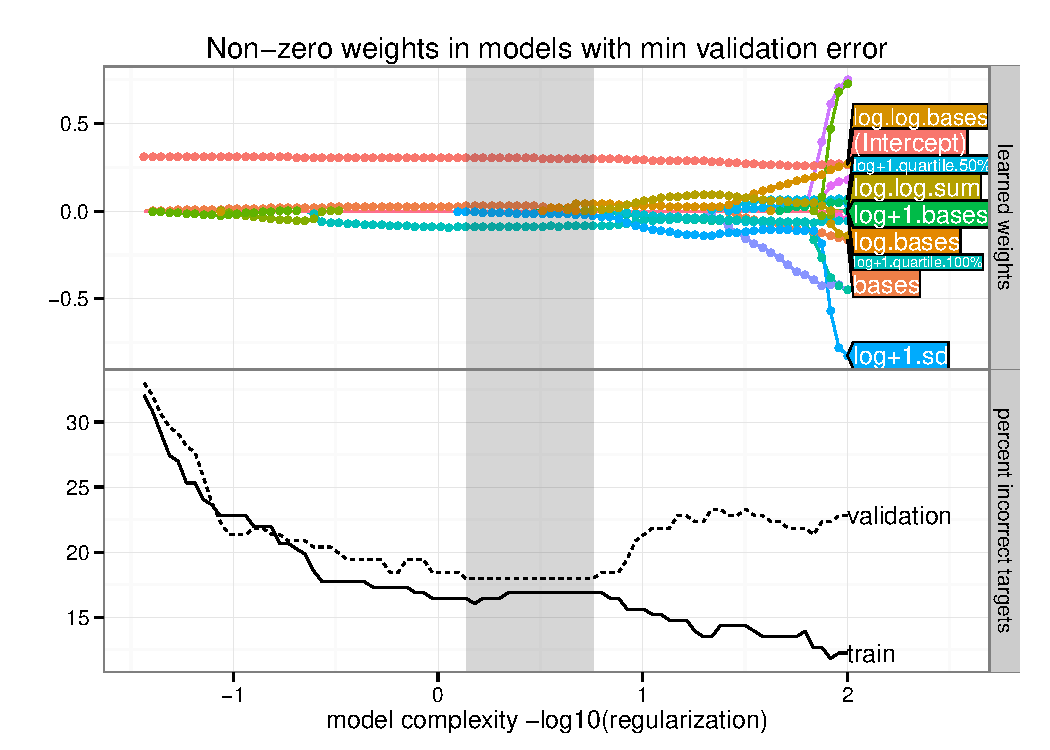
\includegraphics[height=0.9\textheight]{figure-lasso-path}
\end{frame}

\begin{frame}
  \frametitle{Size of positive regions good heuristic for initial grid search}

  \includegraphics[height=0.8\textheight]{figure-label-problem-size}

  6 train/test splits per data set.
\end{frame}

\end{document}
